% !TeX spellcheck = russian-aot
%\documentclass[12pt,a4paper,draft]{article}
%\usepackage{cmap}
%\usepackage[utf8]{inputenc}
%\usepackage[T2A]{fontenc}
%\usepackage[english,german,russian]{babel}
%\usepackage{amsmath}
%\usepackage{amsfonts}
%\usepackage{amssymb}
%\usepackage[final]{graphicx}
%\DeclareGraphicsExtensions{.jpg,.png}
%\graphicspath{{pictures/}} % путь к графическим файлам. Пусть они помещаются в подкаталог pictures текущего каталога
%\usepackage[figurename=Рисунок,labelsep=period]{caption}
%\usepackage{float}
%\usepackage{indentfirst}
%\usepackage[pdftex,left=2.5cm,right=2.5cm,top=3cm,bottom=3cm]{geometry}
%\usepackage[obeyDraft]{todonotes}
%\usepackage[hidelinks,draft=false]{hyperref}
%\frenchspacing
%\pdfcompresslevel=9

\documentclass[a4paper,12pt]{article}
\usepackage[utf8]{inputenc}
\usepackage[T2A]{fontenc}
\usepackage[english,russian]{babel}
\usepackage{natbib}
\usepackage[final]{graphicx}
\DeclareGraphicsExtensions{.jpg,.png}
\graphicspath{{pictures/}}
\usepackage{float}
\usepackage{amsmath}
\usepackage{pgfplots}
\usepackage{color} %% это для отображения цвета в коде
%\usepackage{listings} %% собственно, это и есть пакет listings




%\setmonofont{Consolas} %to be used with XeLaTeX or LuaLaTeX
\definecolor{bluekeywords}{rgb}{0,0,1}
\definecolor{greencomments}{rgb}{0,0.5,0}
\definecolor{redstrings}{rgb}{0.64,0.08,0.08}
\definecolor{xmlcomments}{rgb}{0.5,0.5,0.5}
\definecolor{types}{rgb}{0.17,0.57,0.68}

\usepackage{listings}
\lstset{
language=[Sharp]C,
captionpos=t,
%numbers=left, %Nummerierung
%numberstyle=\tiny, % kleine Zeilennummern
frame=lines, % Oberhalb und unterhalb des Listings ist eine Linie
showspaces=false,
showtabs=false,
breaklines=true,
showstringspaces=false,
breakatwhitespace=true,
escapeinside={(*@}{@*)},
commentstyle=\color{greencomments},
morekeywords={partial, var, value, get, set},
keywordstyle=\color{bluekeywords}\bf,
stringstyle=\color{redstrings},
basicstyle=\ttfamily\small,
extendedchars=\true
}

\usepackage{caption}
\DeclareCaptionFont{white}{\color{white}} %% это сделает текст заголовка белым
%% код ниже нарисует серую рамочку вокруг заголовка кода.
\DeclareCaptionFormat{listing}{\colorbox{gray}{\parbox{\textwidth}{#1#2#3}}}
\captionsetup[lstlisting]{format=listing,labelfont=white,textfont=white}


\usepackage{ctable}%для таблиц
\captionsetup[table]{justification=raggedleft,singlelinecheck=off}




%%%%%%%%%%%%%%%%%%%%%%%%%%%%%%%%%%%%%%%%%%%%%%%%%%%%%%%%%%%%%%%%%%%%%%%%%%%%%%%%%%%%%%%%%%%%%%%

\begin{document}
\begin{titlepage}
	\centering
    \begin{figure}[H]
    	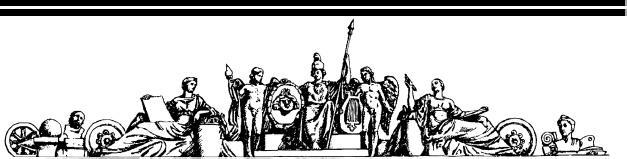
\includegraphics[scale=1.2]{photo}
   	\end{figure}
	{\scshape Министерство образования Российской Федерации
Московский Государственный Технический Университет им. Н.Э. Баумана \par}
	\vspace{4cm}
	{\scshape\Large Отчёт по лабораторной работе № 1\par}
    {\scshape\Large По курсу: "Анализ алгоритмов"\par}
	{\scshape\Large\bf Тема:"Умножение матриц"\par}
    \vspace{4cm}
    {\flushright Студент: Орехова Е.О. ИУ7-51\par
    \flushright Преподаватель: Волкова Л.Л.\par}
    \vspace{3cm}
% Bottom of the page
	{\large \today\par}
\end{titlepage}

\def\contentaname{Содержание}
\tableofcontents %Вывод содержания
\clearpage

\section{Постановка задачи}
    В ходе выполнения лабораторной работы необходимо реализовать умножение матриц обычным алгоритмом и алгоритмом Винограда. Улучшить алгоритм Винограда. Сравнить эти алгоритмы.

\section{Умножение матриц}
    Пусть даны две матрицы, $A$ и $B$, размерности $a \times n$ и $n \times b$ соответственно, тогда результатом их умножения будет матрица $C$, размерности $a \times b$, в которой
    \begin{equation}
    	C_{i,j} = \sum_{k = 1}^{n} A_{i,k}*B{k,j}
    \end{equation}
\section{Алгоритм Винограда}
	Если посмотреть на результат умножения двух матриц, то видно, что каждый элемент в нем представляет собой скалярное произведение соответствующих строки и столбца исходных матриц. Можно заметить также, что такое умножение допускает предварительную обработку, позволяющую часть работы выполнить заранее. Рассмотрим два вектора $V = (v_1,v_2,v_3,v_4)$ и $W = (w_1,w_2,w_3,w_4)$. Их скалярное произведение равно 
	\begin{equation}
		V*W = v_1w_1 + v_2w_2 + v_3w_3 + v_4w_4
	\end{equation}
	Это равенство можно переписать в виде:
	\begin{equation}
	V*W = (v_1+w_2)(v_2+w_1)+(v_3+w_4)(v_4+w_3)-v_1v_2-v_3v_4-w_1w_2-w_3w_4
	\end{equation}
	Из этого следует, что произведение матриц можно выполнить эффективнее, произведя некоторые вычисления заранее.
	
    
\section{Реализация}
\begin{lstlisting}[label=some-code,caption={Стандартный алгоритм умножения матриц}]
public static void Simple_Multiplication(ref int[,]C, int[,] A, int[,] B, int size)
{
	for (int i = 0; i < size; i++)
		for (int j = 0; j < size; j++)
		{
			C[i, j] = 0;
			for (int k = 0; k < size; k++)
				C[i, j] = C[i, j] + A[i,k] * B[k,j];
		}
}
\end{lstlisting}

\begin{lstlisting}[label=some-code1,caption={Алгоритм Винограда}]
public static void Vinograd(ref int[,] C,int[,] A, int[,] B, int size, int [] Rows, int [] Column)
{
	
	for (int i = 0; i < size; i++)
	{
		Rows[i] = A[i, 0] * A[i, 1];
		for (int j = 1; j < size/2; j++)
			Rows[i] = Rows[i]+ A[i, 2 * j] * A[i, 2 * j + 1];
	}
	
	
	for (int i = 0; i < size; i++)
	{
		Column[i] = B[0, i] * B[1, i];
		for (int j = 1; j < size/2; j++)
			Column[i] = Column[i]+ B[2 * j, i] * B[2 * j + 1, i];
	}
	
	
	for(int i = 0; i< size; i++)
		for (int j = 0; j<size;j++)
		{
			C[i, j] = -Rows[i] - Column[j];
			for (int k = 0; k < size/2; k++)
				C[i, j] = C[i, j]+(A[i,2*k+1]+B[2*k,j]) * (A[i,2*k]+B[2*k+1,j]);
		}
	if (size % 2 == 1)
	{
		for (int i = 0; i < size; i++)
			for (int j = 0; j < size; j++)
				C[i, j] = C[i, j]+ A[i,size-1] * B[size-1,j];
	}
}
\end{lstlisting}

\begin{lstlisting}[label=some-code1,caption={Улучшенный алгоритм Винограда}]
public static void Vinograd_Better(ref int[,] C, int[,] A, int[,] B, int size, int[] Rows, int[] Column)
{
	int d = size / 2;
	int new_size = size - 1;
	
	for (int i = 0; i < size; i++)
	{
		Rows[i] = A[i, 0] * A[i, 1];
		for (int j = 2; j < new_size; j+=2)
			Rows[i] += A[i, j] * A[i, j + 1];
	}
	
	for (int i = 0; i < size; i++)
	{
		Column[i] = B[0, i] * B[1, i];
		for (int j = 2; j < new_size; j+=2)
			Column[i] += B[j, i] * B[j + 1, i];
	}
	
	if (size % 2 == 1)
	{
		for (int i = 0; i < size; i++)
			for (int j = 0; j < size; j++)
			{
				C[i, j] = -Rows[i] - Column[j] + A[i, size - 1] * B[size - 1, j];
				for (int k = 0; k < d; k++)
					C[i, j] += (A[i, 2 * k + 1] + B[2 * k, j]) * (A[i, 2 * k] + B[2 * k + 1, j]);
			}
	}
	else
	{
		for (int i = 0; i < size; i++)
			for (int j = 0; j < size; j++)
			{
				C[i, j] = -Rows[i] - Column[j];
				for (int k = 0; k < d; k++)
					C[i, j] += (A[i, 2 * k + 1] + B[2 * k, j]) * (A[i, 2 * k] + B[2 * k + 1, j]);
			}
	}
}
\end{lstlisting}

\section{Теоретическая оценка}
Операции, имеющие сложность 1: +, -, * ,/, <, >, <=, >=, =, ==, +=, -=, /=, *=, []

Размер исходных матриц $N \times N$.

\subsection{Стандартный алгоритм:} 
\begin{gather*}
	f = 2+N(2+2+N(2+3+2+N(2+11))) = 2+4N+N^2(7+13N)=\\*=2+4N+7N^2+13N^3
\end{gather*}

\subsection{Алгоритм Винограда:} 
в лучшем случае:
\begin{gather*}
	f_{best} = 2(2+N(2+6+3+\frac{N}{2}(2+12)))+2+N(2+2+N(2+7+3+N(2+22)))+2 = \\* = 24N^3+26N^2+26N+8
\end{gather*}
в худшем случае:
\begin{gather*}
	f_{worst} = f_{best}+2+N(2+2+N(2+13)) = 24N^3+41N^2+30N+10
\end{gather*}

\subsection{Улучшенный алгоритм Винограда:}
Эффективность алгоритма улучшена следующими операциями:
\begin{enumerate}
	\item Для сокращения операций в цикле в начале алгоритма вычисляется $d = \frac{N}{2}$.
	\item Операции вида $x = x + k$ заменены на $x += k$.
	\item Проверка на четность выполняется вначале цикла.
\end{enumerate}
Общая часть:
\begin{gather*}
	f = 2+2+2(2+N(2+7+2+\frac{N}{2}(2+8)))+2= 10+22N+10N^2
\end{gather*}
в худшем случае:
\begin{gather*}
f_{worst} = f + 2+N(2+2+N(2+15+2+\frac{N}{2}(2+20))) = \\*= f+2+4N+19N^2+11N^3=12+26N+29N^2+11N^3
\end{gather*}
в лучшем случае:
\begin{gather*}
f_{best} = f+2+N(2+2+N(2+7+2+\frac{N}{2}(2+20)))=f+2+4N+11N^2+11N^3=\\*=12+26N+22N^2+11N^3
\end{gather*}


\section{Эксперимент}

\begin{figure}[H]
	\noindent\centering{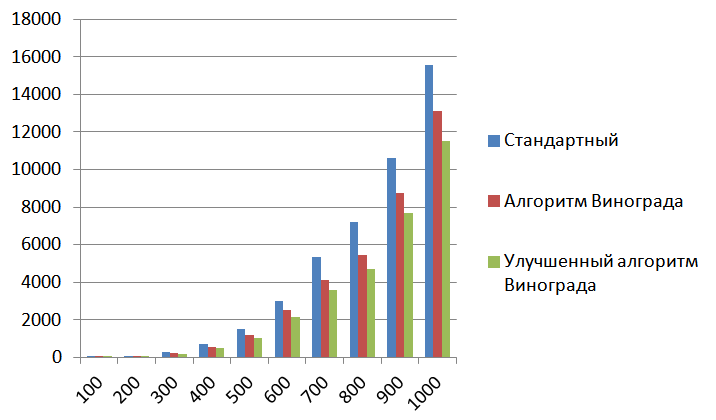
\includegraphics[scale = 1]{file}}
	\caption{Время умножения матриц в мс.}
\end{figure}

\begin{figure}[H]
	\noindent\centering{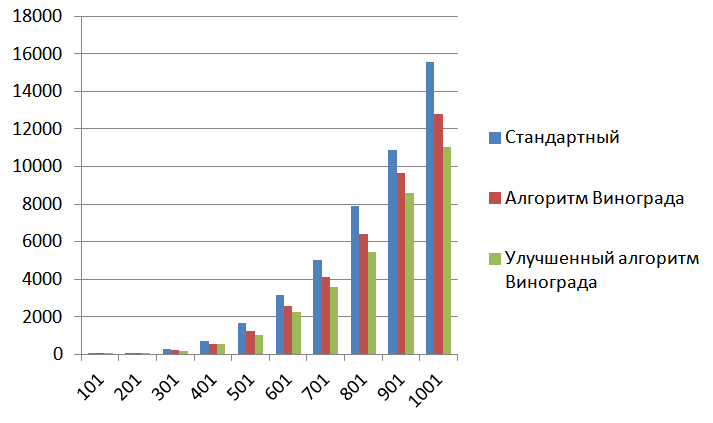
\includegraphics[scale = 1]{file1}}
	\caption{Время умножения матриц в мс.}
\end{figure}

Из диаграмм видно, что алгоритм Винограда выполняется быстрее, несмотря на то, что имеет большую сложность. Это можно объяснить тем, что реальная сложность умножения относительно сложения на вычислительной машине отличается от теоретической. Поэтому алгоритм Винограда работает быстрее.

\section{Заключение}
	В ходе выполнения лабораторной работы были изучены и реализованы различные алгоритмы умножения матриц. Получены временные характеристики.
\end{document} 